% !TEX program = xelatex

\documentclass[hyperref, UTF8,11pt,a4paper]{ctexart} %只有10,11,12磅三个选项
\usepackage[utf8]{inputenc}
\usepackage{amsmath}
\usepackage{amsfonts}
\usepackage{amssymb}
\usepackage{float} % 图像浮动
\usepackage[xetex]{graphicx} % xetex驱动
\usepackage[left=1.00cm, right=0.00cm, top=0.20cm, bottom=0.00cm]{geometry}
\usepackage{color} % 颜色
\title{数学笔记}	% 标题
\author{于洋}			% 作者
\date{}					% 日期
\linespread{1.5}	%行间距
\usepackage[breaklinks,colorlinks,linkcolor=black,citecolor=black,urlcolor=black]{hyperref} % 生成书签
\setlength{\parindent}{0pt}  % 设置缩进

\begin{document}
\maketitle

\newpage

%=========== [ 三角函数 ] =======================================
\section{三角函数}

%=========== 终边一点 ===========================================
\subsection{终边一点}
{\color{red} 角$\alpha$ 终边上一点(-4,3):} \\
$\cos \alpha=\frac{x}{r}=\frac{x}{\sqrt{x^{2}+y^{2}}}=\frac{-4}{\sqrt{(-4)^{2}+3^{2}}}=-\frac{4}{5}$ \\
$\sin \alpha=\frac{y}{r}=\frac{y}{\sqrt{x^{2}+y^{2}}}=\frac{3}{\sqrt{(-4)^{2}+3^{2}}}=\frac{3}{5}$

%=========== 平移================================================

\subsection{平移}
{\color{red}  $\sin \left(2 x+\frac{\pi}{3}\right)$ 移动变成 $\sin \left(2 x+\frac{\pi}{6}\right)$:} \\
1) 提括号:	$\sin \left[2\left(x+\frac{\pi}{6}\right)\right]$ \quad $\sin \left[2\left(x+\frac{\pi}{12}\right)\right]$ \\
2) 相减:$\left(x+\frac{\pi}{12}\right)-\left(x+\frac{\pi}{6}\right)=-\frac{\pi}{12}$ \\
3) 翻译: $-\frac{\pi}{12}$ 是 向右移动 $\frac{\pi}{12}$

%=========== sin和cos 互化 =======================================

\subsection {sin和cos 互化}

$\cos \left(2 x+\frac{\pi}{3}\right) = sin\left(2 x+\frac{\pi}{3}+\frac{\pi}{2}\right)$  \quad 根据 $\cos x=\sin \left(x+\frac{\pi}{2}\right)$ \\
$\sin \left(2 x+\frac{\pi}{3}\right) = cos\left(2 x+\frac{\pi}{3}-\frac{\pi}{2}\right)$  \quad 根据 $\sin x=\cos \left(x-\frac{\pi}{2}\right)$

%=========== 区间内最值,值域=======================================

\subsection{区间内最值,值域}

%figure参数:h 此处(here)t 页顶(top)b 页底(bottom)p 独立一页(page)
\begin{minipage}[h]{0.5\linewidth}
	{\color{red}   $f(x)=4 \sin \left(2 x-\frac{\pi}{3}\right)+\sqrt{3}$在$\left[0, \frac{\pi}{2}\right]$上的最大值,最小值 } \\
	$x \in\left[0, \frac{\pi}{2}\right]$ \\
	2$x \in[0, \pi]$ \\
	$2 x-\frac{\pi}{3} \in\left[-\frac{\pi}{3}, \frac{2}{3} \pi\right]$ \\
	如图此区间的最小值$-\frac{\sqrt{3}}{2}$,最大值1,所以 \\
	$ \sin\left(2 x-\frac{\pi}{3}\right) \in\left[-\frac{\sqrt{3}}{2}, 1\right]$ \\
	$4 \sin \left(2 x-\frac{\pi}{3}\right) \in[-2 \sqrt{3}, 4]$ \\
	$4 \sin \left(2 x-\frac{\pi}{3}\right)+\sqrt{3} \in[-\sqrt{3}, 4+\sqrt{3}]$
\end{minipage}
\hfill
\begin{minipage}[h]{0.5\linewidth}
	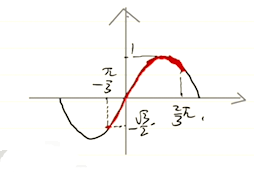
\includegraphics[scale=0.8]{pic/sanjiaohanshu/qujianneizuizhi.png}
\end{minipage}

%=========== 伸缩变换=============================================

\subsection {伸缩变换}
$y = \cos x$ \\
横坐标缩短到原来的$ \frac{1}{2} $ (x换成2x) $\longrightarrow$ $y= \cos 2x$ \\
纵坐标伸长到原来的2倍 (A换成2A) $\longrightarrow$ $y=  2 \cos 2x$ \\
向左平移 $\frac {\pi}{4} $  (x换成 x+4) $\longrightarrow$ $y=2 \cos \left[2\left(x+\frac{\pi}{4}\right)\right]$
%=========== 对称中心,对称轴,单调区间 =============================

\subsection {对称中心,对称轴,单调区间}

{\color{red}  $y=\sin \left(2 x-\frac{\pi}{3}\right)$ 的减区间} \\
\begin{figure}[h] %figure参数:h 此处(here)t 页顶(top)b 页底(bottom)p 独立一页(page)
	\begin{center}
		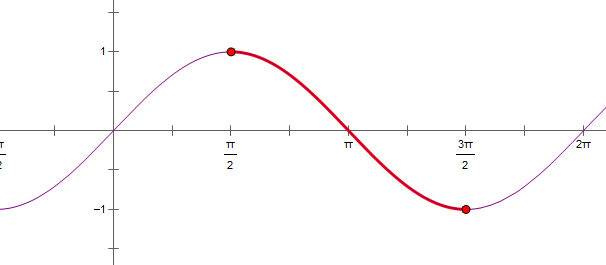
\includegraphics[scale=0.3]  {pic/sanjiaohanshu/dandiaojianqujian.png}
		\caption{$\sin x$ 减区间}
	\end{center}
\end{figure}


与基础图形对照:
\begin{tabular}{|c|c|}
	\hline
	$\sin x$ 减区间                              & $x \in\left[\frac{\pi}{2}+2 k \pi, \frac{3}{2} \pi+2 k \pi\right](k \in z)$                 \\
	\hline
	$\sin \left(2 x-\frac{\pi}{3}\right)$ 减区间 & $2 x-\frac{\pi}{3} \in\left[\frac{\pi}{2}+2 k \pi, \frac{3}{2} \pi+2 k \pi\right](k \in z)$ \\
	\hline
\end{tabular} \\
计算出$x$范围 . {\color{red}  对称中心,对称轴,同样原理,都是根据基础图形,替换即可}

%==============     sinx图像翻转 =================================
\subsection {sinx图像翻转}
$y=|\sin x|$ , $y=\sin |x|$ , $y=-\sin x$ 图像 \\
\begin{figure}[htbp]
	\begin{center}
		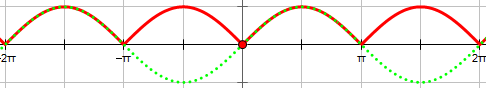
\includegraphics[scale=0.6]  {pic/sanjiaohanshu/abs(sin(x)).png}
		\caption{y=$|\sin x|$ $\qquad$ \textbf{整体加绝对值: x轴下方图像翻折到上方. 下方图像不保留.}  }
		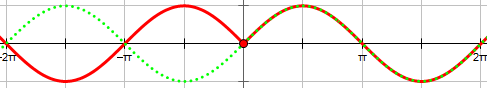
\includegraphics[scale=0.6]  {pic/sanjiaohanshu/sin(abs(x)).png}
		\caption{y=$\sin |x|$ $\qquad$\textbf{x加绝对值: 先画出 x 轴正半轴,再沿y轴翻折.}}
		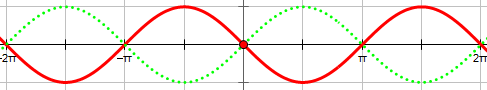
\includegraphics[scale=0.6]  {pic/sanjiaohanshu/-sinx.png}
		\caption{y=$-\sin x$ $\qquad$\textbf{整体加负号: 沿x轴上下翻折.}}
	\end{center}

\end{figure}

%==============     零点个数 =====================================
\subsection {零点个数}
{\color{red}  $f(x)=\left(\frac{1}{2}\right)^{x}-\sin x$ 零点个数} \\
令 $f(x)=0$ 即$\left(\frac{1}{2}\right)^{x}=\sin x$ \\
画出等号左右两侧图像,交点个数就是零点个数 (2个)
\begin{figure}[h] %figure参数:h 此处(here)t 页顶(top)b 页底(bottom)p 独立一页(page)
	\begin{center}
		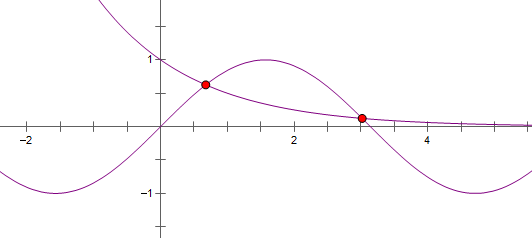
\includegraphics[scale=0.5]  {pic/sanjiaohanshu/lingdiangeshu.png}
		\caption{$f(x)=\left(\frac{1}{2}\right)^{x}$ , $f(x)=\sin x$}
	\end{center}
\end{figure}

\newpage
%==============  [ 正余弦 ]=======================================
\section{正余弦}
%==============  正弦定理(多解取舍) ===============================
\subsection{正弦定理(多解取舍)}
{\color{red} 在 $\Delta A B C$中,$b=\sqrt{3}, B=60^{\circ}, c=1$,求C } \\
$ \frac{b}{\sin B}=\frac{c}{\sin C} \therefore \sin C=\frac{1}{2}, c=30^{\circ}$或$150^{\circ}$ \\
角度取舍两种思路:\\
1) 依据大边对大角:  \quad
$\because b>c,  \therefore B<C \therefore C=30^{\circ}$ \\
2) 三角形内角和 $180^{\circ}$ : \quad
$ \because   B=60^{\circ}, \therefore 0^{\circ}<C<120^{\circ}  \therefore C=30^{\circ}$ \\

%============= 角化边,边化角,角化角 ===============================

\subsection{角化边,边化角,角化角}
{\color{red} $3a\cos A=c\cos B+b\cos C$,求$\cos A $} \\
两种思路都可以: \\
边 $\rightarrow$ 角 \\
$3 \sin A \cos A=\sin C \cos B+\sin B \cos C =\sin (B+C) =\sin A$
$\therefore   \cos A=\frac{1}{3}$ \\
角 $\rightarrow$ 边	 \\
$3 a \cos A=c \cdot \frac{a^{2}+c^{2}-b^{2}}{2 a c}+b \cdot \frac{a^{2}+b^{2}-c^{2}}{2 a b}$
$\therefore  \cos A=\frac{1}{3}$ \\

%============= 判断三角形形状 =====================================

\subsection{三角形形状(讨论n种情况)}

\begin{figure}[htbp] %figure参数:h 此处(here)t 页顶(top)b 页底(bottom)p 独立一页(page)
	\centering
	\begin{minipage}{170pt}
		\centering
		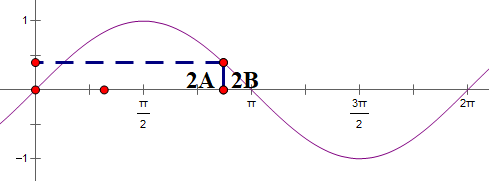
\includegraphics[width=170pt]  {pic/zhengyuxian/2A=2B.png}
		\caption{2A=2B}
	\end{minipage}
	\hspace{10pt}
	\begin{minipage}{170pt}
		\centering
		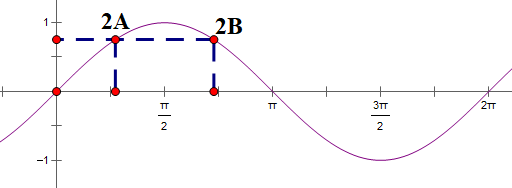
\includegraphics[width=170pt]  {pic/zhengyuxian/2A=2B1.png}
		\caption{$ 2A+2B= \frac{\pi}{2} * 2 $}
	\end{minipage}
	\hspace{10pt}
	\begin{minipage}{170pt}
		\centering
		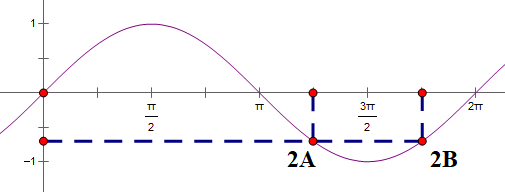
\includegraphics[width=170pt]  {pic/zhengyuxian/2A=2B2.png}
		\caption{$ 2A+2B= \frac{3\pi}{2} * 2 $}
	\end{minipage}
\end{figure}

{\color{red} $ \sin 2A= \sin 2B$ } \\

$\because 0<A<\pi \therefore 0<2A<2\pi$ \\
如图:三种情况 \\
1) 当$ 2A=2B $时 等腰三角形 \\
2) 当$ 2A+2B= \frac{\pi}{2} * 2 $ 时, 直角三角形 \\
3) 当$ 2A+2B= \frac{3\pi}{2} * 2 $ 时, 不符合三角形 \\




\subsection{已知三边判断三角形形状}
{\color{red} 已知三角形三边为 3,5,7 求三角形是形状(锐角,直角,钝角) } \\
$\because 3^{2}+5^{2}<7^{2}$ $\therefore$ 钝角

%============= [ 向量 ] ==========================================
\section{向量}

%============= [ 绝对值 ] ==========================================

\subsection{绝对值}
{\color{blue} 绝对值、想平方,算完之后不要慌. }\\
{\color{red}  题目: } \\
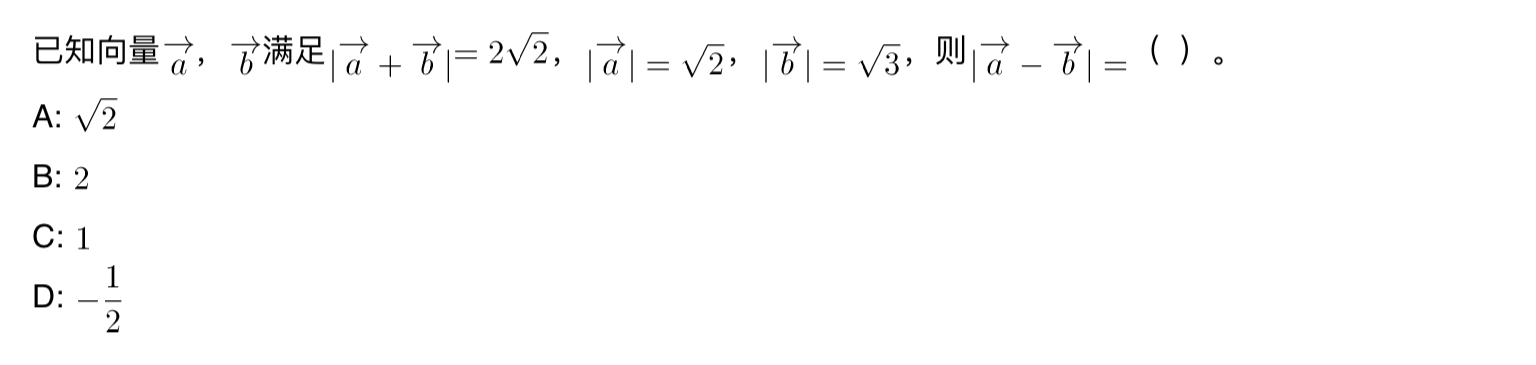
\includegraphics[width=500pt]  {pic/xiangliang/jueduizhi.jpg} \\
解答: A\\
$\because |\vec{a}+\vec{b}|^{2}=|\vec{a}|^{2}+|\vec{b}|^{2}+2 \vec{a} \cdot \vec{b}=8$ \\
$ \therefore 2 \vec{a} \cdot \vec{b}=3$ \\
$\therefore |\vec{a}-\vec{b}|^{2}=|\vec{a}|^{2}+|\vec{b}|^{2}-2 \vec{a} \cdot \vec{b}=2$ \\

%============= [ 夹角锐角钝角 ] =======================================

\subsection{夹角锐角钝角}
% {\color{blue} 绝对值、想平方,算完之后不要慌. }\\
{\color{red}  题目: } \\

\includegraphics[width=500pt]  {pic/xiangliang/jiajiaotimu.jpg} \\
解答: {\color{blue}  $\vec{a} \cdot \vec{b}>0$ 且 不共线} \\
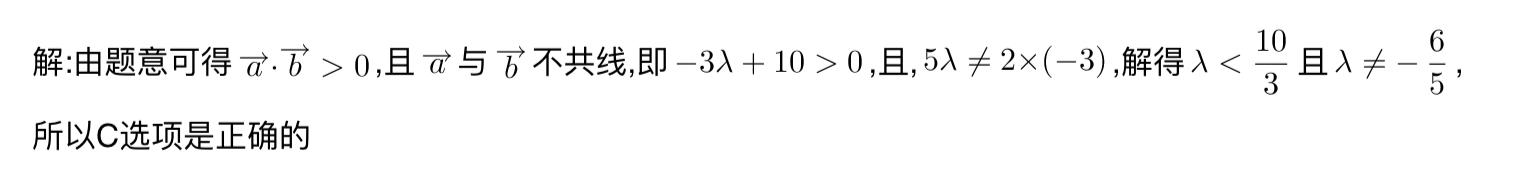
\includegraphics[width=500pt]  {pic/xiangliang/jiajiaojieda.jpg} \\

%============= [ 基础图形(理) ] ==========================================

\subsection{基础图形(理)}
{\color{red}  题目: } \\


%============= [ 基底建模法 ] ==========================================

\subsection{基底建模法(理)}
{\color{red}  题目: } \\
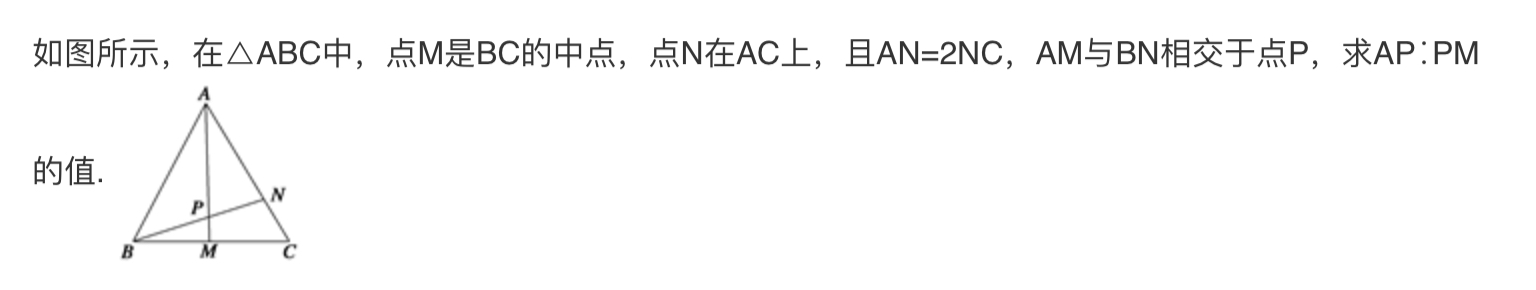
\includegraphics[width=500pt]  {pic/xiangliang/jidijianmofa.jpg} \\
解答:{\color{blue} 以$\overrightarrow{B M}$,$\overrightarrow{C N}$为基底,进行计算.} \\
设:$e_{1}=\overrightarrow{B M}, \quad e_{2}=\overrightarrow{C N}$,则 \\ \\
$\overrightarrow{A M}=\overrightarrow{A C}+\overrightarrow{C M}=-3 e_{2}-e_{1}$ \\
$\overrightarrow{B N}=\overrightarrow{B C}+\overrightarrow{C N}=2 e_{1}+e_{2}$ \\
因为A,P,M和B,P,N分别共线 所以:\\ \\
$\overrightarrow{A P}=\lambda \overrightarrow{A M}=-\lambda e_{1}-$ 3$\lambda e_{2}$ \\
$\overrightarrow{B P}=\mu \overrightarrow{B N}=2 \mu e_{1}+\mu e_{2}$ \\ \\
$\overrightarrow{B A}=\overrightarrow{B P}-\overrightarrow{A P}=(\lambda+2 \mu) e_{1}+(3 \lambda+$ $\mu ) e_{2}$ \\
$\overrightarrow{B A}=\overrightarrow{B C}+\overrightarrow{C A}=2 e_{1}+3 e_{2}$ \\ \\
$\left\{\begin{array}{l}{\lambda+2 \mu=2} \\ {3 \lambda+\mu=3}\end{array}\right.$
$\left\{\begin{array}{l}{\lambda=\frac{4}{5}} \\ {\mu=\frac{3}{5}}\end{array}\right.$ \\
$\therefore A P : P M=4 : 1$


\newpage
%============= [ 数列 ] ==========================================
\section{数列}

%============= [ 分式数列 ] ======================================

\subsection{分式数列 单调性}
{\color{red} 数列 $a_{n}=\frac{n-\sqrt{2016}}{n-\sqrt{2017}}$,则前100项的最大项,最小项是第几项 }\\
解:$a_{n}=\frac{n-\sqrt{2016}}{n-\sqrt{2017}}=1+\frac{\sqrt{2017}-\sqrt{2016}}{n-\sqrt{2017}}$ \\
根据函数图像: \\
当 $n \in[1,44]$ 时,$\left\{a_{n}\right\}$单调递减, \\
当 $n \in[45,+\infty)$ 单调递增, \\
$\therefore \left(a_{n}\right)_{\max }=a_{45},\left(a_{n}\right)_{\min }=a_{44}$

%============= [ 分段数列 ] ======================================

\subsection{分段数列 单调性}
{\color{red}  题目: } \\
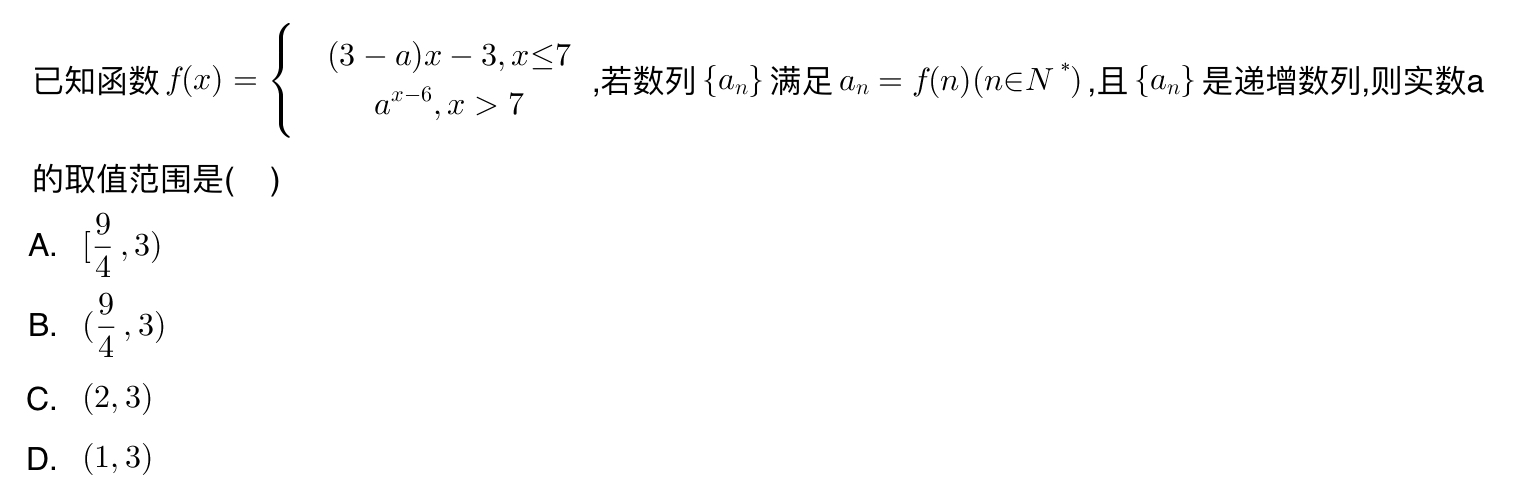
\includegraphics[width=500pt]  {pic/shulie/fenduanhanshutimu.jpg} \\
解答: \\
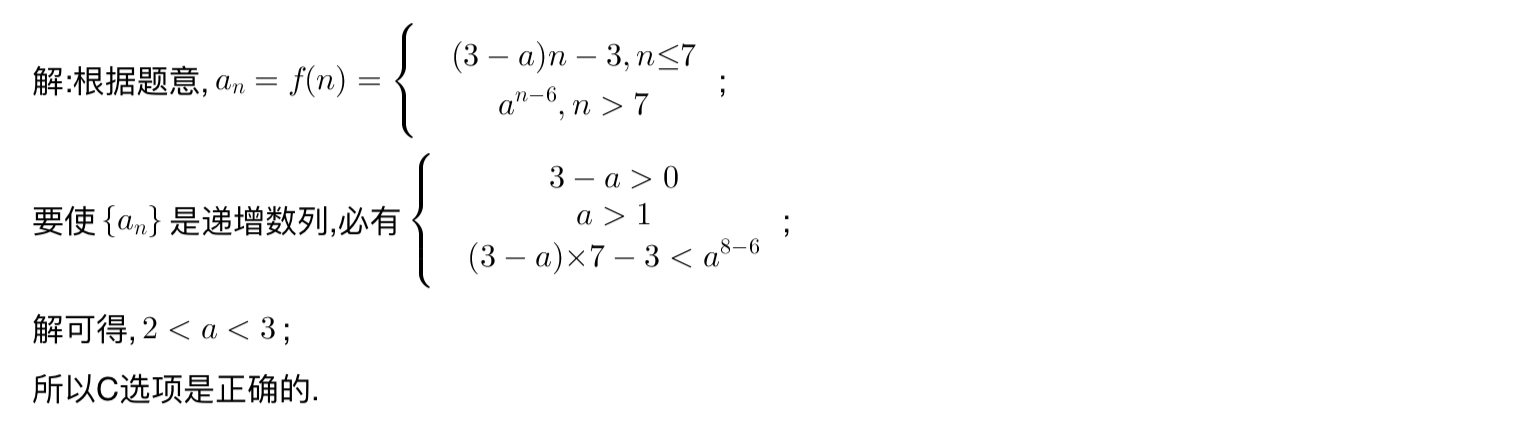
\includegraphics[width=500pt]  {pic/shulie/fenduanhanshudaan.jpg} \\

%============= [ 一般数列 ] ======================================

\subsection{一般数列 单调性}
{\color{red}  题目: } \\
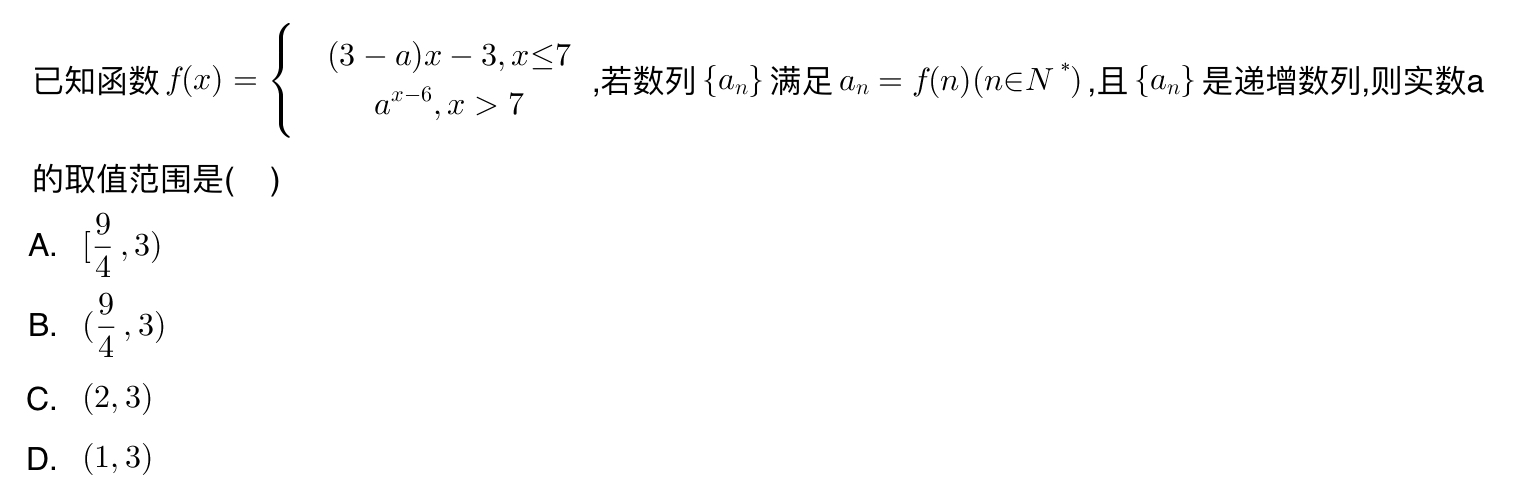
\includegraphics[width=500pt]  {pic/shulie/fenduanhanshutimu.jpg} \\
解答: \\
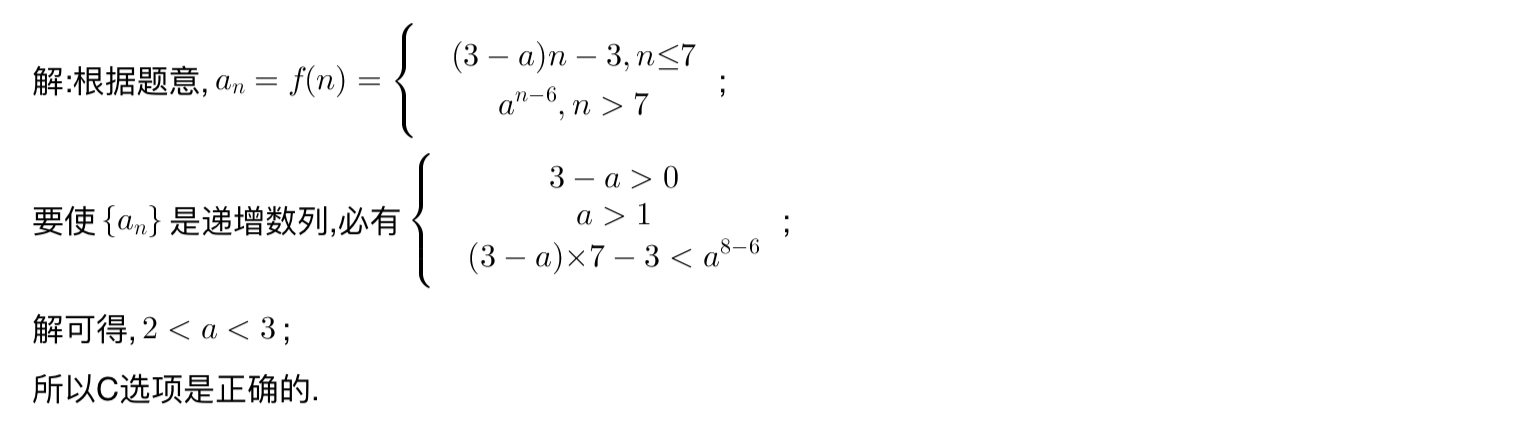
\includegraphics[width=500pt]  {pic/shulie/fenduanhanshudaan.jpg} \\

\end{document}
